\documentclass[12pt]{article}
\usepackage{fullpage, amsmath, amssymb, amsthm, amscd, setspace, bm, graphicx, indentfirst, multirow, tikz, enumerate}
\usepackage{adjustbox,amsfonts,array,graphicx,booktabs,tabularx,multirow,multicol,stmaryrd, tabu}
\usepackage[utf8]{inputenc}
\usetikzlibrary{arrows.meta}
\title{Math 412, Fall 2023 -- Homework 6}
\date{}
\setlength{\parskip}{0.5cm}
\setlength{\parindent}{0cm}

\newtheorem{theorem}{Theorem}[section]
\newtheorem{definition}[theorem]{Definition}
\newtheorem{lemma}[theorem]{Lemma}
\newtheorem{proposition}[theorem]{Proposition}
\newtheorem{corollary}[theorem]{Corollary}
\newtheorem{remark}[theorem]{Remark}
\newtheorem{example}[theorem]{Example}

\newcommand{\Z}{\mathbb{Z}}
\newcommand{\R}{\mathbb{R}}
\newcommand{\Q}{\mathbb{Q}}
\newcommand{\C}{\mathbb{C}}
\newcommand{\ba}{\overline}
\newcommand{\Hom}{\text{Hom}}
\newcommand{\End}{\text{End}}
\newcommand{\wt}[1]{\text{wt}({#1})}
\begin{document} \maketitle
\vspace{-80pt}

\textbf{Due:} Wednesday, October 11th, at 9:00AM via Gradescope

\textbf{Instructions:} Students taking the course for three credit hours (undergraduates, most graduate
students) should choose four of the following five problems to solve and turn in--if you do all five, only the first four will be graded. Graduate students
taking the course for four credits should solve all five. Problems that use the word ``describe”,
``determine”, ``show", or ``prove" require proof for all claims.

\begin{enumerate}

\item[1.] Consider the following graph.

    \begin{center}
        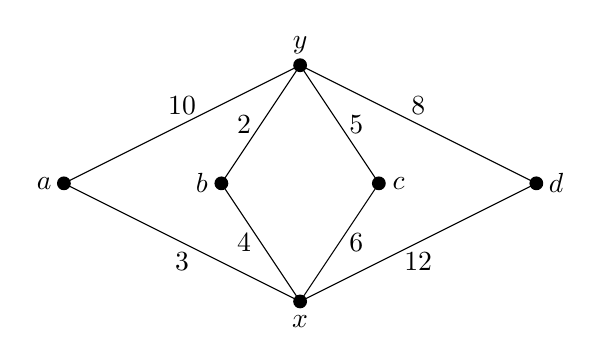
\begin{tikzpicture}
            \draw [line width=0.25mm, fill=black] (0,0) circle (0.75mm);
            \draw [line width=0.25mm, fill=black] (0,3) circle (0.75mm);
            \draw [line width=0.25mm, fill=black] (-3,1.5) circle (0.75mm);
            \draw [line width=0.25mm, fill=black] (-1,1.5) circle (0.75mm);
            \draw [line width=0.25mm, fill=black] (1,1.5) circle (0.75mm);
            \draw [line width=0.25mm, fill=black] (3,1.5) circle (0.75mm);
            \draw (0,0) to node[midway,below]{$3$} (-3,1.5);
            \draw (-3,1.5) to node[midway,above]{$10$} (0,3);
            \draw (0,0) to node[midway,left]{$4$} (-1,1.5);
            \draw (-1,1.5) to node[midway,left]{$2$} (0,3);
            \draw (0,0) to node[midway,right]{$6$} (1,1.5);
            \draw (1,1.5) to node[midway,right]{$5$} (0,3);
            \draw (0,0) to node[midway,below]{$12$} (3,1.5);
            \draw (3,1.5) to node[midway,above]{$8$} (0,3);
            \node at (0,-0.25) {$x$};
            \node at (0,3.25) {$y$};
            \node at (-3.25,1.5) {$a$};
            \node at (-1.25,1.5) {$b$};
            \node at (1.25,1.5) {$c$};
            \node at (3.25,1.5) {$d$};
        \end{tikzpicture}
    \end{center}

\begin{enumerate}
    \item[(a)] Use Kruskal's algorithm to construct a minimal spanning tree, and find its weight. Show your work step by step: which edge is considered at each step of the algorithm, is it accepted or rejected, and why?
    
    \item[(b)] Use Dijkstra's algorithm to find the distance from $y$ to every vertex. Again, show your work step by step, including the set $S$ and the values of the function $t$ at each step.
    
\end{enumerate}

\item[2.] For any spanning tree $T$ in a weighted graph $G$, let \[m(T) = \max_{e\in E(T)} \wt{e}.\] Further, let \[x(G) = \min_T m(T),\] where the minimum is over all spanning trees of $G$.

\begin{enumerate}

\item[(a)] If $T$ is a minimal spanning tree of $G$, prove that $m(T) = x(G)$.

\item[(b)] Give an example of a graph $G$ and a \emph{non-minimal} spanning tree $T$ such that $m(T)= x(G)$.

\end{enumerate}

\item[3.] Let $G$ be an $X,Y$-bigraph, i.e. a bipartite graph whose partite sets are $X$ and $Y$. If $|X|=|Y|$, prove that there exists a subset $S\subseteq X$ with $|N(S)|<|S|$ if and only if there exists a subset $T\subseteq Y$ with $|N(T)|<|T|$.

\item[4.] Let $G$ be a graph. Prove that the number of edges in every maximal matching in $G$ is at least half the number of edges of a maximum matching of $G$.

\item[5.] Let $D$ be a digraph. Prove that there exist pairwise disjoint cycles in $D$ such that each vertex of $D$ lies in exactly one of the cycles if and only if \[|N^+(S)|\ge |S| \text{ for all } S\subseteq V(D).\]

\end{enumerate}




\end{document}
